
%(BEGIN_QUESTION)
% Copyright 2015, Tony R. Kuphaldt, released under the Creative Commons Attribution License (v 1.0)
% This means you may do almost anything with this work of mine, so long as you give me proper credit

\noindent

\vskip 5pt



I dette arbeidsoppdraget skal du sette i drift nivåregulering på en stasjon. Du skal prøve optimalisere PID parametrene på følgende måter\begin{itemize}[noitemsep]
\item Z\&N svingemetode
\item Skogestads metode
\end{itemize}
I dette arbeidsoppdraget skal du sette i drift strømningsregulering på en stasjon. Du skal prøve optimalisere PID parametrene på følgende måter\begin{itemize}[noitemsep]
\item Z\&N svingemetode
\item Skogestads metode
\item Lærerens jukse metode
\end{itemize}



%$$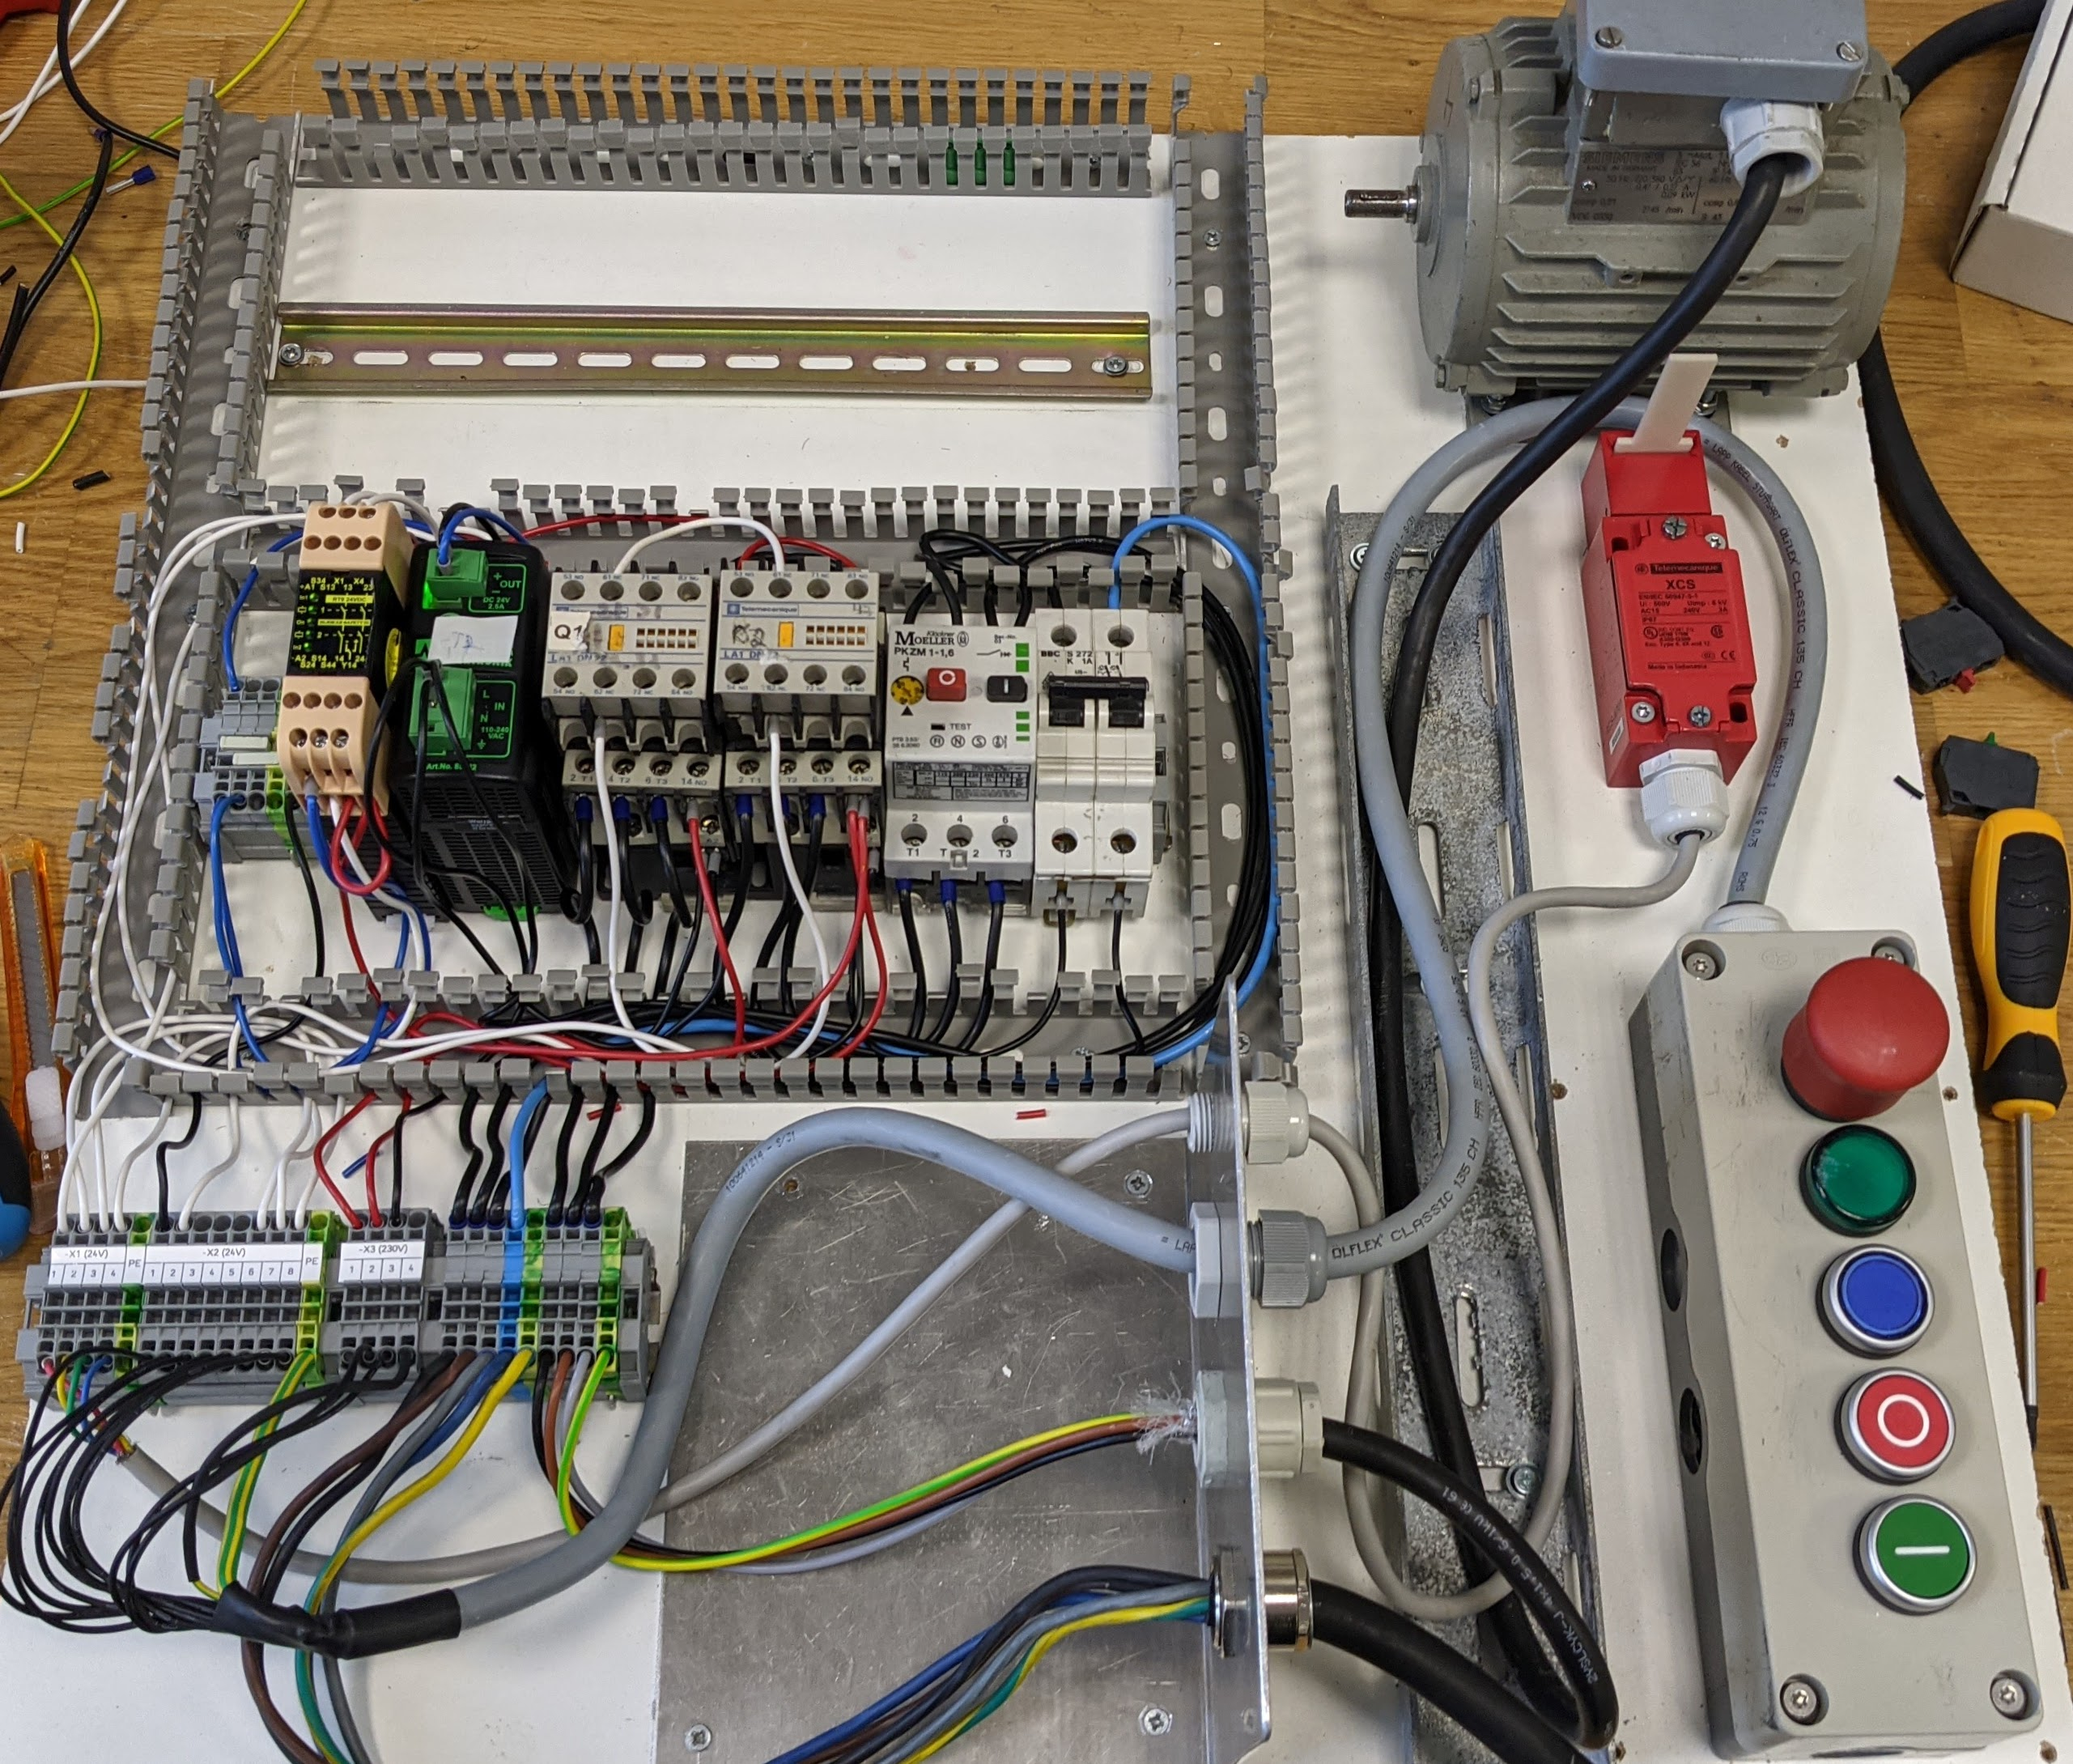
\includegraphics[width=13cm]{i04821x01.jpg}$$\\
\textbf{Teorioppgaver}

\textbf{Planlegging}

\textbf{Gjennomføring}

\textbf{Dokumentasjon}

Lag et dokument som viser hvordan du gikk frem for å optimalisere med de ulike metodene. 















\underbar{file i04857}
\vfil \eject
%(END_QUESTION)





%(BEGIN_ANSWER)


%(END_ANSWER)





%(BEGIN_NOTES)


%INDEX% Arbeisdoppdrag, Kompetanse, Nivå 1, Stasjonxx, Mal

%(END_NOTES)


